A Support Vector Machine(SVM) is a classifier which outputs an optimal hyperplane or set of hyperplanes in high-dimensional space and classifies data. A hyperplane in a n-dimensional space, is a subspace of one dimension less than the whole space. In figure \ref{fig:SVM} a hyperplane in 2-dimensional space is a line which divides the 2-dimensional space in half. This division defines two closed half-space, and represents the division between two classes. The original idea for SVM was conceived by Cortes and Vapnik in 1995 \cite{cortes1995support} \\
In figure \ref{fig:SVM}, the main idea behind SVM is shown. Consider for example a dataset described by variables $x_1$ and $x_2$ and suppose we want to classify all the elements(elements are shown by class circle and class square), then the operation of an SVM algorithm is based on finding the optimal hyperplane between the two classes \cite{opencv_library}. An optimal hyperplane is one that gives the largest minimum distance to the classes and it maximizes the margin between the hyperplane and all data points. %i.e. the best line that leaves the maximum margin from both classes.

\begin{figure}[H]
    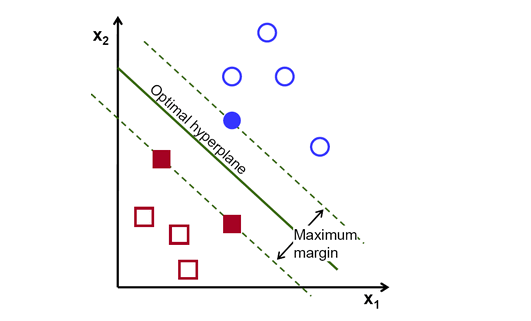
\includegraphics[width=0.45\textwidth]{./img/SVM.png}
    \caption{\footnotesize{SVM with a Maximum-margin hyperplane and margins trained with samples from two classes circle and square. Samples on the margin are called the support vectors.\cite{wiki:SVM}}}
    \label{fig:SVM}
\end{figure}


SVM are popular for numerous theoretical reasons: SVM classifiers are robust to very large number of variables. They have strong founding theory and need less memory to store the predictive model; Even when training samples have some bias, when the right parameters are chosen for an SVM, then it can be robust\cite{auria2008support} and can learn both simple and complex classification models \cite{cristianini2000}. 


SVMs are the best known member in the general category of kernel methods. Kernel methods are a class of algorithms often used in pattern analysis which can operate on general types of data(e.g strings, vector, text) and looks for general relations between data points (ranking, classification, clusters). The modular framework of Kernel Methods is shown in figure\ref{fig:Kernel}. In the first step, data points are processed in a vector space(kernel matrix) through a mapping function(kernel function). Second, different kernel algorithms can be used in order to analyze the data, using only the information that resides in the kernel matrix. \cite{shawe2004kernel}\\

%This allows the user to apply a classifier to data that has infinite- dimensional vector space representation such as DNA or protein \cite{ben2010user}. \\

\begin{figure}[H]
	\centering
    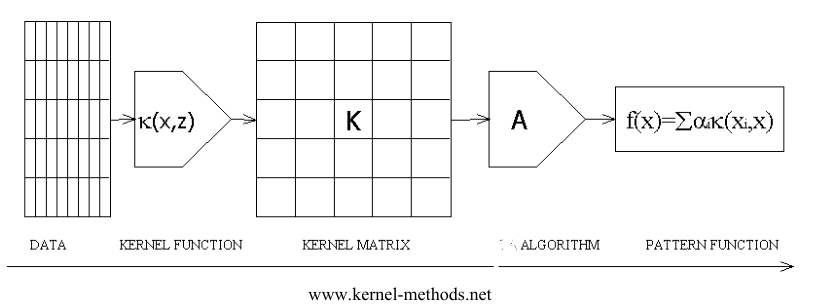
\includegraphics[width=0.35\textwidth]{./img/kernel1.png}
     \caption{\footnotesize{Modeular framework of Kernel methods }}
    \label{fig:Kernel}
\end{figure} 



In recent years, SVMs are widely used in bio-informatics \cite{furey2000support,osuna1997training,guyon2002gene} and other disciplines due to its ability to accurately deal with high dimensional data\cite{joachims1998text}. In marine environments, researchers have proposed a method for detection of oil spills in SAR images, using SVM as a classifier. A study has shown that SVM has better performance on SAR images when using a texture analysis and decomposition algorithm in various steps of the SVM algorithm. Texture analysis will help to reduce noise in SAR images \cite{matkan2013oil}.



